\documentclass[conference]{IEEEtran}
\IEEEoverridecommandlockouts
% The preceding line is only needed to identify funding in the first footnote. If that is unneeded, please comment it out.
\usepackage{cite}
\usepackage{amsmath,amssymb,amsfonts}
\usepackage{algorithmic}
\usepackage{graphicx}
\usepackage{textcomp}
\usepackage{xcolor}
\usepackage{booktabs}
\def\BibTeX{{\rm B\kern-.05em{\sc i\kern-.025em b}\kern-.08em
    T\kern-.1667em\lower.7ex\hbox{E}\kern-.125emX}}
\begin{document}

\title{Multi-modal MRI for Identifying Lymphovascular Invasion in Endometrial Cancer\\}

\author{
\IEEEauthorblockN{Puzhu Wang}
\IEEEauthorblockA{
\textit{LSA Statistics Department} \\
\textit{University of Michigan} \\
Ann Arbor, USA \\
puzhu@umich.edu
}
}

\maketitle

\begin{abstract}
Magnetic resonance imaging (MRI)-based radiomics has been widely explored for preoperative prediction of lymphovascular invasion (LVI) in endometrial cancer. This study investigates LVI prediction from multi-modal MRI radiomic features (T1, T2, and ADC) of two clinical centers under both supervised and unsupervised frameworks, with explicit center harmonization. We find that center~2 consists of two technically distinct acquisition batches, one of which contains no LVI-positive patient, so that acquisition batch and outcome are confounded. Without harmonization, logistic regression with T1+T2 features reaches a test AUC of 0.93, reproducing earlier results. After ComBat harmonization by acquisition batch, fitted on training data only, the cross-validated AUC falls from 0.89 to 0.83, and within a single center it is only 0.68. Single-modality spectral clustering shows that the previously reported label-pure clusters coincide with acquisition batches, and that no stable cluster structure remains after harmonization. Adaptive gated fusion networks do not improve on simpler fusion and overfit the harmonized data. These results indicate that a substantial part of the apparent LVI signal in this dataset is technical, and they motivate batch-aware validation and an external cohort before MRI radiomics is used for LVI prediction.
\end{abstract}

\section{Introduction}
Magnetic resonance imaging (MRI) is the preferred modality for preoperative evaluation of endometrial cancer, primarily for staging purposes such as assessing myometrial invasion depth and cervical stromal involvement \cite{ma2025predictive}. These factors are essential for guiding treatment decisions, including fertility preservation and the extent of surgical intervention.

Lymphovascular invasion (LVI) is a major prognostic factor, second only to myometrial invasion depth, and plays an important role in surgical planning, adjuvant therapy decisions, and prognosis. However, LVI is a microscopic pathological feature and cannot be directly visualized by MRI, as lymphovascular structures are far below the spatial resolution of standard imaging.
Current European guidelines combine LVI status with histotype, grade, depth of myometrial invasion and molecular classification to define the risk groups that determine the extent of lymph-node staging and the indication for adjuvant therapy \cite{concin2021esgo}. Because LVI is only confirmed on the surgical specimen, a reliable preoperative imaging surrogate would let this information guide surgical planning rather than only postoperative management.

Despite this limitation, it is of interest to investigate whether multi-modal MRI-derived features (T1, T2, and ADC) can provide indirect information related to LVI. Previous studies have shown that MRI-based traditional radiomics and computer-vision nomogram are useful for LVI prediction and may facilitate better clinical decision-making \cite{long2021mri}. In particular, we examine whether LVI-positive and LVI-negative patients exhibit distinct patterns in high-dimensional feature space, and whether these patterns persist once technical differences between centers are removed.

In the literature on MRI-based LVI prediction, the least absolute shrinkage and selection operator (LASSO) is one of the most widely used methods for feature selection \cite{liu2024multimodal} \cite{luo2020multiparametric}. In addition, sequential feature selection procedures, such as the Mann–Whitney U test, Spearman correlation filtering, and stepwise regression, are commonly employed depending on the study design. For prediction, traditional models including support vector machines (particularly with RBF kernels), random forests, and logistic regression with LASSO or ridge regularization are frequently adopted \cite{liu2024multimodal} \cite{huang2022multi}.

Radiomics rests on the premise that medical images contain quantitative information about tumor phenotype beyond what is visible to the radiologist \cite{gillies2016radiomics}. Its clinical translation, however, depends on reproducible feature definitions and on robustness to differences in acquisition. The Image Biomarker Standardization Initiative has standardized feature definitions and their computation \cite{zwanenburg2020ibsi}, and quality frameworks such as the radiomics quality score emphasize multicenter validation, calibration and the control of technical variation \cite{lambin2017radiomics}. Radiomic features are sensitive to scanner, protocol, reconstruction and preprocessing settings \cite{mali2021radiomics}. ComBat, an empirical Bayes method that removes batch-specific location and scale effects \cite{johnson2007combat}, has become the standard statistical harmonization for multicenter imaging features \cite{fortin2018cortical,orlhac2018postreconstruction,orlhac2022guide}. Two caveats are central here: the batch should be the acquisition setting that generates the technical shift rather than simply the hospital \cite{orlhac2022guide}, and when batch is confounded with the outcome, no harmonization can separate the two, while protecting the outcome in the ComBat model inflates downstream significance \cite{nygaard2016methods,leek2010tackling}. Most published MRI models for LVI pool one or two centers without explicitly assessing such effects \cite{luo2020multiparametric,long2021mri,liu2024multimodal}.

However, multi-modal MRI data (T1, T2, and ADC) cannot be effectively utilized by these traditional models without explicit fusion strategies. Methods such as SVM, random forest, and logistic regression do not inherently account for modality-specific contributions, and their fusion mechanisms are typically predefined rather than learned from data. To address this limitation, adaptive gated fusion networks provide a flexible framework for learning modality-specific and patient-specific representations and dynamically combining them \cite{zhou2025agfnet}.
More generally, multimodal machine learning distinguishes early (feature-level), late (decision-level) and intermediate (representation-level) fusion \cite{baltrusaitis2019multimodal}. Early fusion is simple but can let a single modality dominate in high-dimensional, small-sample settings, whereas late fusion is more robust to modality-specific noise but cannot model cross-modal interactions \cite{pereira2023comparative}. Gated and attention-based intermediate fusion learn sample-specific modality weights, offering a compromise between the two and a route to interpretability.

In contrast to supervised approaches, there is relatively limited literature on unsupervised learning for MRI-based LVI identification, making it an underexplored yet promising research direction. Nevertheless, relevant methodologies can be drawn from the broader literature on latent space clustering. Classical approaches such as multi-omics factor analysis, along with more recent deep learning methods, including ClusterGAN \cite{mukherjee2019clustergan}, Variational Deep Embedding \cite{jiang2016variational}, and multi-view clustering in latent embedding spaces \cite{chen2020multi}, all provide useful frameworks for modeling heterogeneous and multi-modal data in an unsupervised setting.
Linear latent-variable models such as iCluster and multi-omics factor analysis (MOFA) estimate a low-dimensional representation shared across data types while separating shared from modality-specific variation \cite{shen2009icluster,argelaguet2018mofa,argelaguet2020mofaplus}, and integrative clustering toolkits combine several such algorithms by consensus \cite{lu2020movics}. In multiparametric breast MRI, integrative radiomics clustering has identified patient subgroups that differ in receptor status, tumor size and nodal metastasis \cite{he2024integrative}. Because a clustering algorithm always returns a partition, the number of clusters has to be justified by internal validation: the silhouette width \cite{rousseeuw1987silhouettes}, resampling stability measured by the adjusted Rand index \cite{hubert1985comparing}, and consensus clustering summarized by the proportion of ambiguous clustering (PAC) \cite{monti2003consensus,senbabaoglu2014critical}.

\section{Method}
\subsection{Data and Cohort}

The dataset used in this study was collected by the Affiliated Hospital of Nanjing University of Chinese Medicine from two clinical centers over a specified period, with appropriate patient consent and authorization for public use. The original MRI signals were preprocessed following a multiparametric MRI-based radiomics pipeline \cite{cao2024multiparameter}, implemented by one of the original contributors, Jingya Chen, who is in the Department of Radiology at the Affiliated Hospital of Nanjing University of Chinese Medicine. Each of the T1, T2 and ADC sequences contributes 396 radiomic features.

We exclude patients with missing values in any of the T1-, T2-, or ADC-derived features, which leaves 329 patients (77 LVI-positive). Given the limited sample size, the dataset is split into training (263) and testing (66) sets using a stratified 80–20 ratio. All analyses are implemented as a reproducible Python pipeline with fixed random seeds (Section~\ref{sec:repro}).

\subsection{Center Harmonization}

Exploratory analysis showed that center~2 is not homogeneous: for about one hundred run-length and low-grey-level texture features, 98 of the 160 center-2 patients have values several orders of magnitude larger than all other patients, consistently in T1, T2 and ADC. We define acquisition batches without using the outcome, by the share of such extreme values per patient, which is sharply bimodal. This gives three batches: C1 (center~1, $n=169$, 47 LVI-positive), C2a ($n=62$, 30 LVI-positive) and C2b ($n=98$, no LVI-positive patient).

We compare four preprocessing settings for each modality: (i) the original raw z-score; (ii) a log (strictly positive features) or Yeo–Johnson transform followed by standardization, without harmonization; (iii) the same transform followed by ComBat \cite{johnson2007combat} with hospital center as batch; and (iv) ComBat with acquisition batch, which is our primary setting. In settings (ii)–(iv), features whose modal value covers more than 20\% of a batch are removed beforehand, because such near-constant features become batch fingerprints after ComBat. Every transformation, including ComBat, is fitted on the training set only and applied to the test set with the training estimates, so that harmonization does not leak test information. The outcome is not protected in the ComBat model, because protecting a covariate confounded with batch inflates its apparent effect \cite{nygaard2016methods}. Harmonization is assessed by the share of features that differ in location between batches (Kruskal–Wallis, BH-FDR), the PERMANOVA $R^2$ of batch, and the silhouette of batch labels in the first ten principal components.

\subsection{Explanatory Data Analysis}

We perform feature selection on the training set through a combination of univariate testing and correlation-based filtering. Specifically, the 50 features most associated with the outcome (ANOVA $F$) are retained, and highly correlated features (pairwise correlation coefficient $> 0.8$) are removed to reduce redundancy. The same feature subset selected from the training set is then consistently applied to the test set. To ensure fair comparability across downstream models, we deliberately avoid model-based feature selection methods (e.g., LASSO) at this stage.

Following feature selection, we assess cross-modality consistency at both the global and local levels within the training set. For global agreement, we compute the correlation between within-modality pairwise distance matrices across different modalities. For local structure, we employ t-SNE to visualize and compare neighborhood patterns in the reduced-dimensional space, coloring patients by LVI status and by acquisition batch.

Since the goal of the unsupervised learning is to understand the overall structure of the dataset rather than evaluate predictive generalization, and given the limited sample size, we do not perform a train-test split for it. Each modality is harmonized without labels, standardized and filtered by correlation, without any label information.

\subsection{Supervised Learning}

In the supervised learning setting, we first establish baseline models using logistic regression and soft-margin support vector machines (SVM), both with $L_2$ regularization to mitigate overfitting. We evaluate multiple modality configurations, including single-modality models, pairwise combinations, and full early fusion via feature concatenation of all three modalities. The regularization parameter is selected by 5-fold cross-validated AUC on the training set. To better prioritize clinically critical cases, specifically patients with undetected disease, we further tune the classification threshold to try to reduce the false negative rate, with additional evaluation using the F1 score.

Since early fusion may lead to greater performance degradation and more susceptible to overfitting in small-sample settings, we also consider late fusion strategies \cite{pereira2023comparative}. Specifically, we construct simple late fusion schemes by combining predictions from single-modality models with weights tuned on the training AUC, and compare their performance against early fusion approaches. To improve model flexibility beyond linear decision boundaries, we extend the baseline models to include nonlinear variants, namely RBF-kernel logistic regression and SVM, enabling learning in a richer feature space.

Building upon the baseline models, we explore an adaptive gated fusion network for multi-modal learning. Given the limited sample size, the network is carefully designed to control model complexity and prevent overfitting. In particular, we adopt small hidden layer dimensions (8 or 16 units) and relatively large dropout rates (0.4).

To better understand the contribution of each component, we construct the model in a progressive (ablation study) manner:
\begin{itemize}
    \item Single-modality neural networks to establish neural baselines
    \item Multi-modality fusion network (early fusion) combining all three modalities
    \item Adaptive Global-weight fusion network, where each modality is assigned a learnable global importance weight
    \item Adaptive Gated-weight fusion network, where modality weights are dynamically assigned at the patient level
\end{itemize}
Each network is trained for 200 epochs with Adam and ten random seeds, and we report the mean and standard deviation of the final train and test performance rather than the best run.

Because a single 66-patient test set is noisy, we assess robustness of the logistic-regression results in three further ways: repeated stratified 5-fold cross-validation (10 repeats) over all patients, refitting harmonization, feature selection and tuning inside every fold; cross-validation within center~1 only, a single acquisition batch in which batch cannot be confounded with LVI; and leave-one-center-out validation, in which the model is trained on one center and tested on the other.

\subsection{Unsupervised Learning}
Through exploratory data analysis and the consistent behavior observed across supervised models, we suspect that the dataset may contain (latent) clustering structure. Such heterogeneity may induce natural differences in class separability across subregions of the feature space. In particular, if several highly concentrated subgroups are present, they may disproportionately influence supervised model fitting and prediction.

Our unsupervised analysis here focuses on clustering structure within each single modality. For each modality, we apply spectral clustering (RBF affinity with $\gamma = 1/p$) for $K = 2,\dots,5$ and visualize the resulting cluster assignments using t-SNE. To assess clustering robustness, we repeatedly subsample 80\% of patients (100 replications) and evaluate the stability of cluster assignments using the mean pairwise adjusted Rand index (ARI), and we compute the proportion of ambiguous clustering (PAC) from 50-run consensus matrices. The analysis is performed on both the original and the harmonized features, and each cluster is described by its LVI rate and its acquisition-batch composition. Within the mixed-label cluster, we additionally refit logistic regression to examine whether focusing on the more heterogeneous subset changes predictive performance. Multi-modal latent-space modeling with MOFA, $k$-means consensus clustering and post-hoc clinical analysis are reported separately in the Unsupervised Extension.

\section{Results}
\subsection{Center Harmonization}

\begin{figure*}[t]
\centering
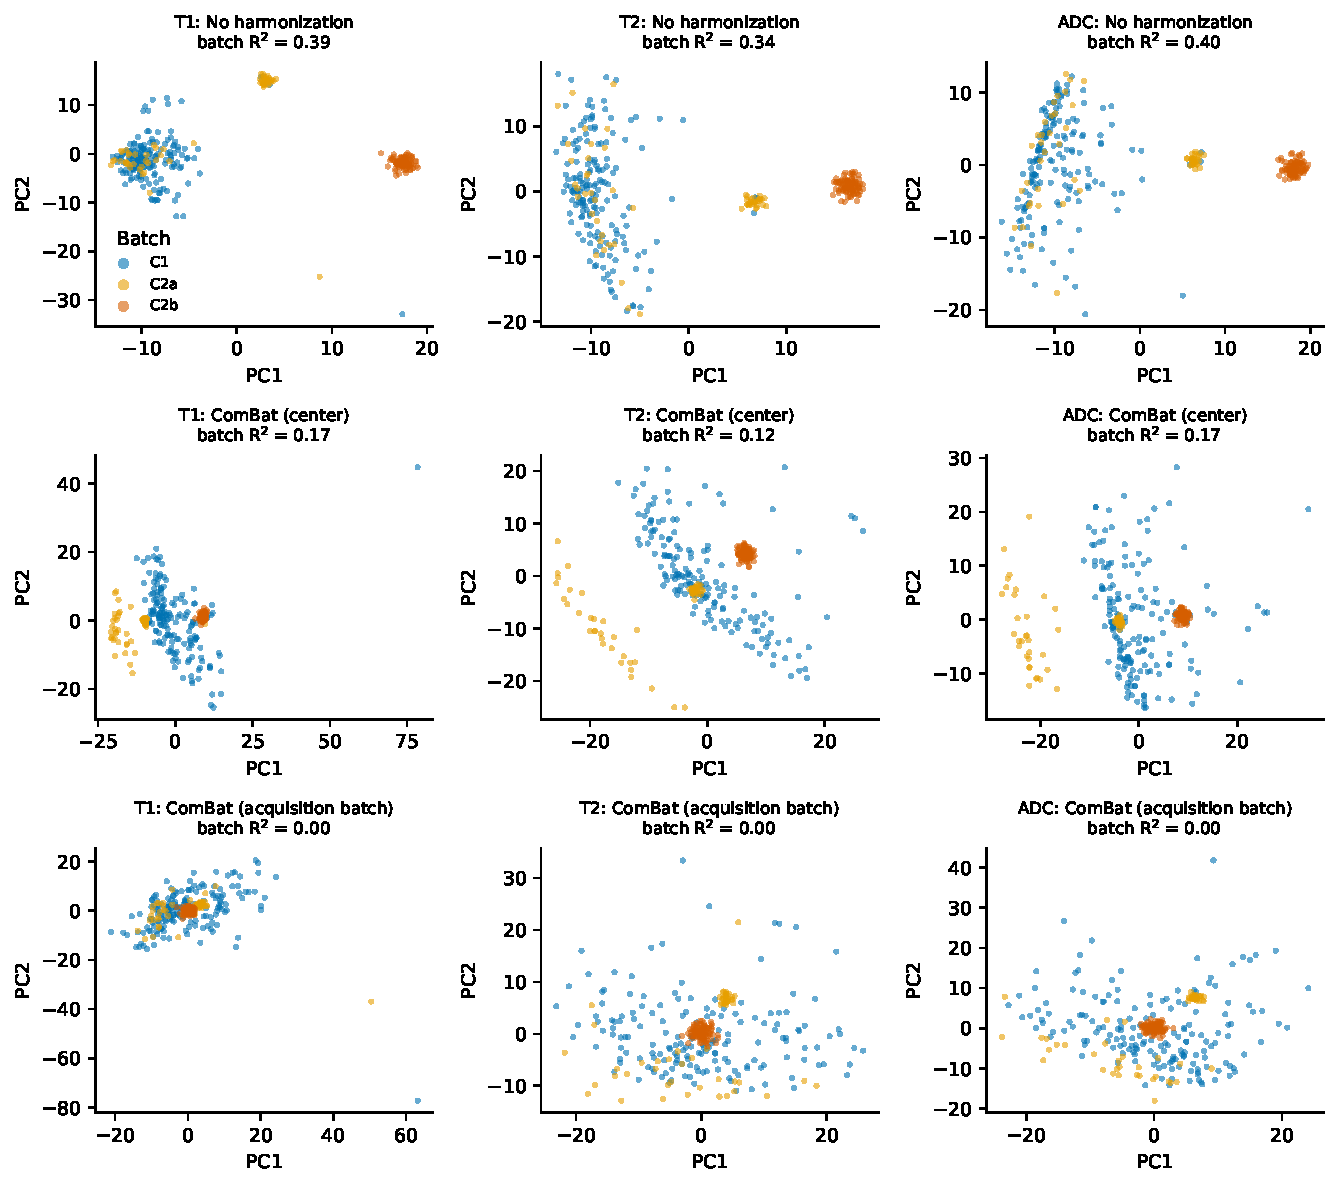
\includegraphics[width=0.85\textwidth]{figures/harmonization_pca.pdf}
\caption{First two principal components of each sequence colored by acquisition batch, without harmonization (top), after ComBat by center (middle) and after ComBat by acquisition batch (bottom); $R^2$: PERMANOVA share of variance explained by batch.}
\label{fig:harm}
\end{figure*}

Without harmonization, acquisition batch explains 34–40\% of the multivariate variance of each sequence, and 93–97\% of features differ in location between batches (Fig.~\ref{fig:harm}). ComBat by hospital center removes the center difference by construction but leaves 12–17\% of the variance and 77–86\% of the features associated with batch, because the two center-2 batches remain. ComBat by acquisition batch reduces the batch $R^2$ to below 0.001, the share of batch-associated features to 3–7\%, and the batch silhouette from about 0.3 to $-0.01$. The detailed tests of harmonization, including higher-order residual effects, are reported in the Unsupervised Extension.

\subsection{Explanatory Data Analysis}

\begin{figure}
\centerline{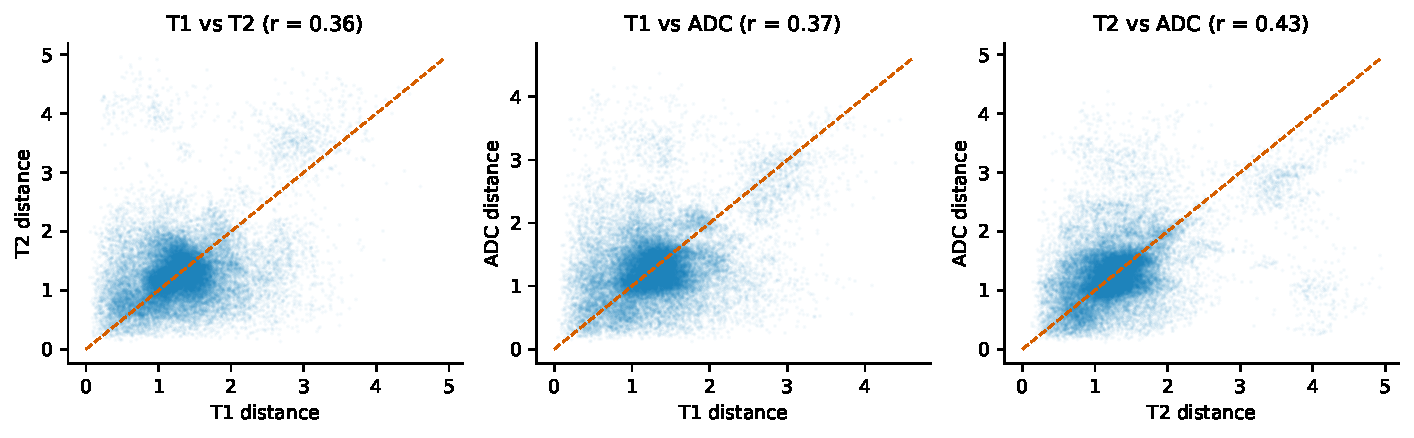
\includegraphics[width=1\columnwidth]{figures/global_agreement_harmonized.pdf}}
\caption{Pairwise global structure agreement after ComBat by acquisition batch (training set).}
\label{fig:global}
\end{figure}

On the original features, the global structure agreement reproduces our earlier observation: correlation coefficients between pairwise distances are 0.45 for T1–T2, 0.23 for T1–ADC and 0.92 for T2–ADC. After harmonization, the three pairs agree to a similar, moderate degree (0.36, 0.37 and 0.43; Fig.~\ref{fig:global}). The very high T2–ADC agreement was therefore largely driven by the batch structure shared by the two sequences rather than by redundant tumor information.

\begin{figure*}[t]
\centering
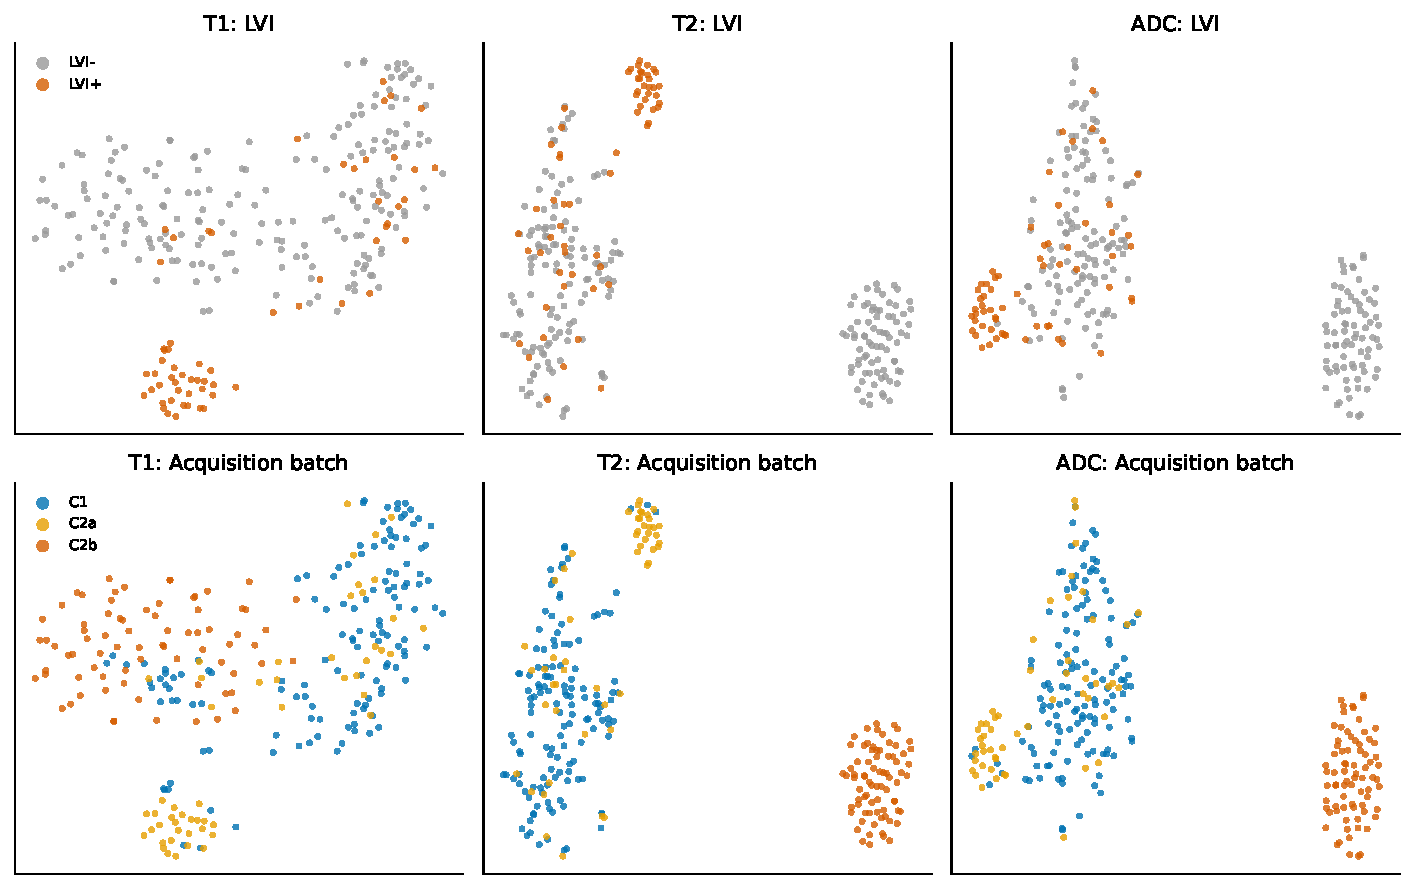
\includegraphics[width=0.8\textwidth]{figures/local_neighborhood_original.pdf}
\caption{Local neighborhood structure (t-SNE, training set, original features), colored by LVI (top) and by acquisition batch (bottom).}
\label{fig:local}
\end{figure*}

The t-SNE visualizations in Fig.~\ref{fig:local} show why. On the original features, the compact and well-separated groups seen in all three modalities coincide with acquisition batches: a large, purely LVI-negative group is batch C2b, and a tight, almost purely LVI-positive group consists of the center-2 LVI-positive patients. After harmonization (Fig.~\ref{fig:local_h}), batch C2b merges with the center-1 patients, but the center-2 LVI-positive patients still form a compact group in every modality. These patients belong to batch C2a and were apparently extracted as a separate block, so their LVI status and their extraction block cannot be separated by harmonization. Elsewhere in the embedding, LVI-positive and LVI-negative patients overlap.

\begin{figure*}[t]
\centering
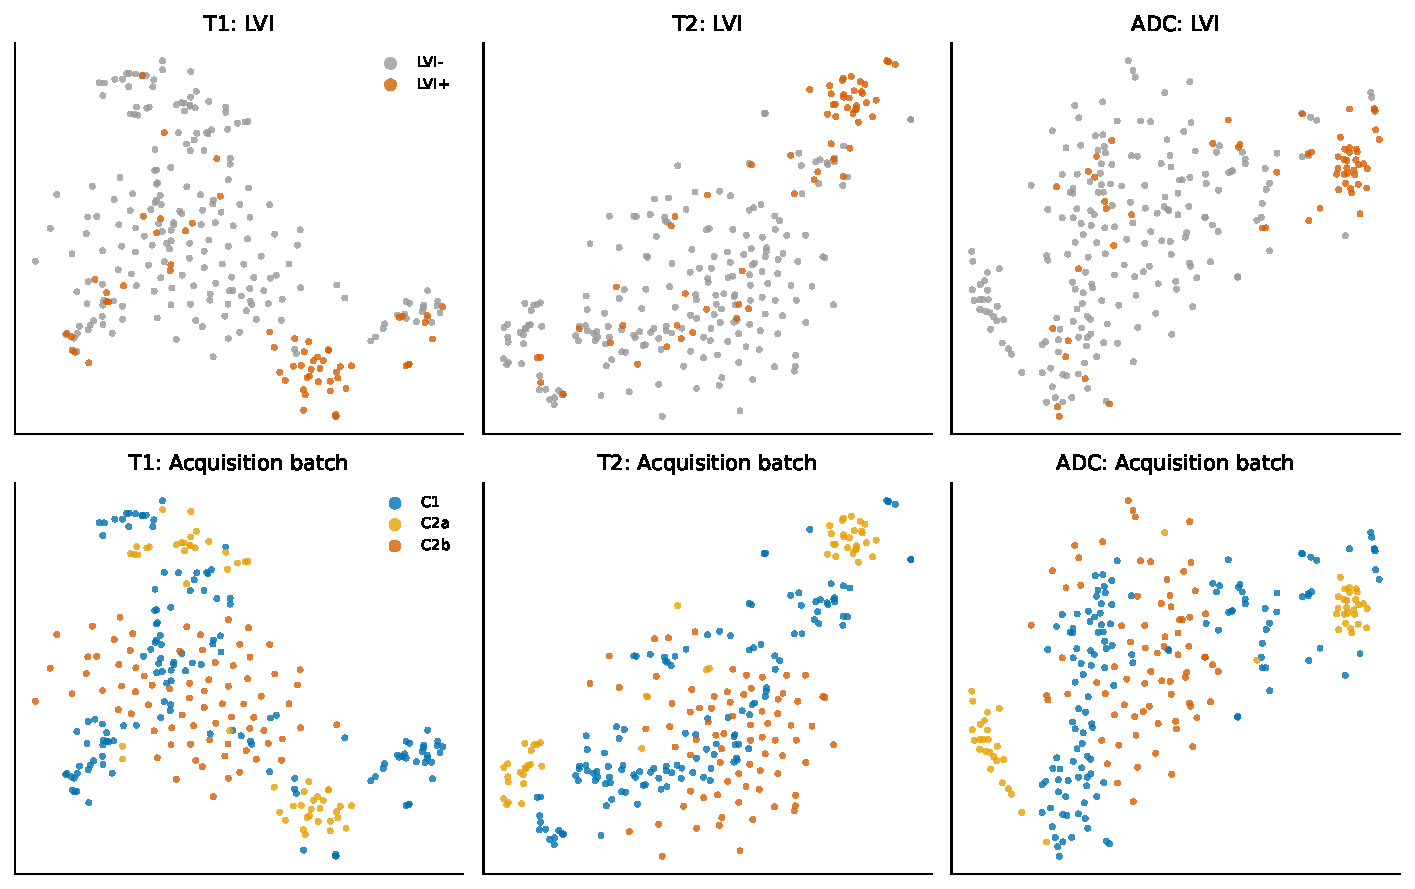
\includegraphics[width=0.8\textwidth]{figures/local_neighborhood_harmonized.pdf}
\caption{Local neighborhood structure (t-SNE, training set) after ComBat by acquisition batch, colored by LVI (top) and by acquisition batch (bottom).}
\label{fig:local_h}
\end{figure*}

\subsection{Supervised Learning}

\begin{figure*}[t]
\centering
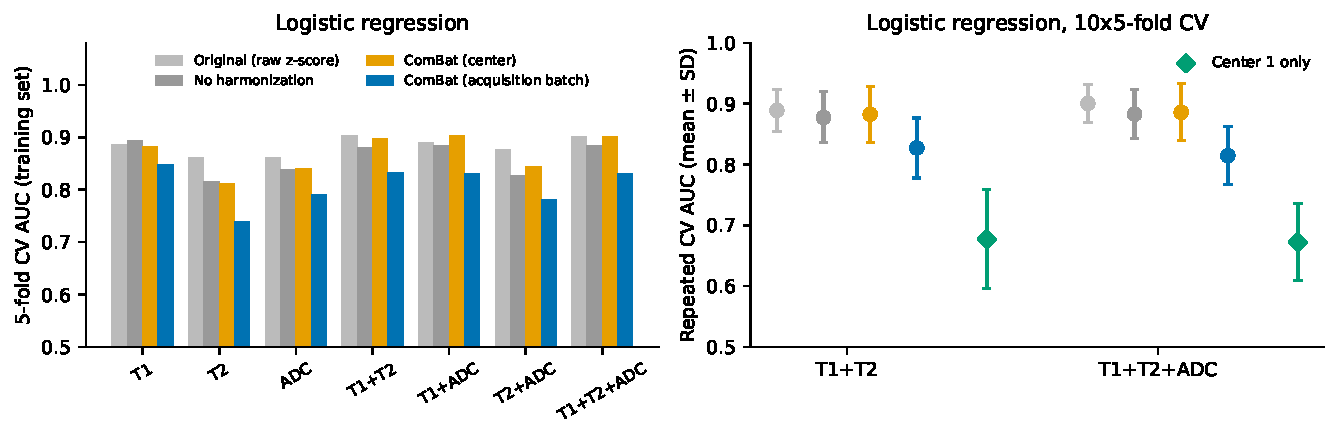
\includegraphics[width=0.85\textwidth]{figures/baseline_harmonization_auc.pdf}
\caption{Logistic regression under the four preprocessing settings. Left: 5-fold cross-validated AUC on the training set for every modality combination. Right: repeated 5-fold cross-validation over all patients (mean $\pm$ SD), with the center-1-only estimate.}
\label{fig:harmauc}
\end{figure*}

\begin{table}[t]
\caption{Best linear baseline per preprocessing setting (selected by training CV AUC) and repeated-CV AUC of logistic regression with T1+T2.}
\label{tab:baselines}
\centering
\footnotesize
\begin{tabular}{lcccc}
\toprule
\textbf{Setting} & \textbf{Best set} & \textbf{CV} & \textbf{Test} & \textbf{Rep.\ CV (T1+T2)}\\
\midrule
Original (raw)    & T1+T2  & 0.90 & 0.93 & $0.89 \pm 0.03$ \\
No harmonization  & T1     & 0.89 & 0.86 & $0.88 \pm 0.04$ \\
ComBat (center)   & T1+ADC & 0.90 & 0.86 & $0.88 \pm 0.05$ \\
ComBat (batch)    & T1     & 0.85 & 0.73 & $0.83 \pm 0.05$ \\
\midrule
Center 1 only     & T1+T2  & \multicolumn{2}{c}{--} & $0.68 \pm 0.08$ \\
\bottomrule
\end{tabular}
\end{table}

On the original features, logistic regression with T1+T2 features again achieves the highest cross-validated AUC (0.90) with consistent training (0.91) and testing (0.93) AUC values, reproducing our earlier results. Harmonization changes this picture (Fig.~\ref{fig:harmauc}, Table~\ref{tab:baselines}). ComBat by center, which leaves the center-2 batches intact, has little effect. ComBat by acquisition batch lowers the cross-validated AUC of every modality combination, most strongly for T2 (from 0.86 to 0.74) and T2+ADC (from 0.88 to 0.78). The best harmonized model is logistic regression on T1 (CV AUC 0.85, test AUC 0.73), and adding T2 or ADC no longer helps. The repeated cross-validation confirms the drop with much less noise than the single split (T1+T2: $0.89 \pm 0.03$ on the original features vs.\ $0.83 \pm 0.05$ after harmonization).

Two further analyses indicate that even the harmonized estimate is optimistic. Within center~1, a single acquisition batch in which batch cannot be confounded with LVI, the cross-validated AUC is only $0.68 \pm 0.08$ for T1+T2 ($0.68$ for T1, $0.57$ for T2 and $0.60$ for ADC). In leave-one-center-out validation, the AUC depends strongly on the direction and the harmonization: training on center~2 and testing on center~1 gives 0.61–0.72, whereas training on center~1 and testing on center~2 ranges from 0.53 without harmonization to 0.98 after batch harmonization. The latter value is implausibly high and reflects the center-2 LVI-positive patients, who form a separately extracted block, being shifted away from the LVI-negative batches. The same block, which harmonization cannot remove, plausibly accounts for much of the gap between the pooled harmonized estimate (0.83) and the center-1 estimate (0.68).

\begin{figure}[t]
\centering
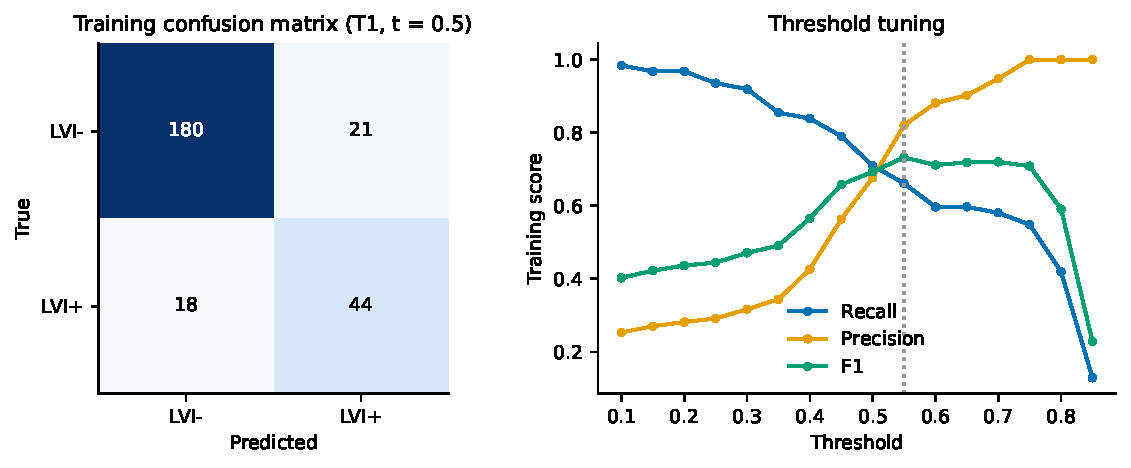
\includegraphics[width=\columnwidth]{figures/baseline_threshold.pdf}
\caption{Best harmonized model (logistic regression, T1). Left: training confusion matrix at threshold 0.5. Right: threshold tuning curve illustrating the trade-off across decision thresholds.}
\label{fig:thresh}
\end{figure}

As before, the model has a relatively high false negative rate (Fig.~\ref{fig:thresh}). Threshold tuning on the training set selects 0.55 (recall 0.66, precision 0.82, F1 0.73). On the test set this threshold yields recall 0.53, precision 0.89 and F1 0.67, missing 7 of 15 LVI-positive patients.

Late fusion models combining all three modalities assign the largest weight to T2 on the original features (weights $0.20/0.60/0.20$) and reach test AUCs of 0.90–0.92; after harmonization their test AUC falls to 0.73–0.75. Similarly, extending models to nonlinear feature spaces using RBF kernels does not yield consistent gains: the best harmonized kernel model (RBF SVM on T1+ADC) reaches a test AUC of 0.79, within the variability of the linear models.

\begin{table}[t]
\caption{Progressive Fusion Network Comparison (mean $\pm$ SD over 10 seeds)}
\label{tab:adaptive_fusion}
\centering
\footnotesize
\begin{tabular}{lcc}
\toprule
\textbf{Model} & \textbf{Original: Test AUC} & \textbf{ComBat: Train / Test AUC}\\
\midrule
Single (T1)       & $0.85 \pm 0.01$ & $0.93$ / $0.75 \pm 0.03$ \\
Single (T2)       & $0.85 \pm 0.02$ & $0.94$ / $0.71 \pm 0.03$ \\
Single (ADC)      & $0.80 \pm 0.01$ & $0.94$ / $0.75 \pm 0.04$ \\
Early fusion      & $0.89 \pm 0.02$ & $0.99$ / $0.85 \pm 0.02$ \\
Adaptive global   & $0.89 \pm 0.01$ & $0.99$ / $0.84 \pm 0.01$ \\
Adaptive gated    & $0.85 \pm 0.05$ & $1.00$ / $0.75 \pm 0.03$ \\
\bottomrule
\end{tabular}
\end{table}

For the progressive fusion networks, we again observe limited gains in predictive performance, as shown in Table~\ref{tab:adaptive_fusion}. On the original features, early and global-weight fusion improve on the single-modality networks (test AUC 0.89), while the gated network is less stable across seeds ($0.85 \pm 0.05$). On the harmonized features, the networks fit the training data almost perfectly (train AUC 0.99–1.00) and their test AUC falls to 0.75–0.85, a clear sign of overfitting in this sample size; the gated network performs worst.

\begin{figure}[t]
\centering
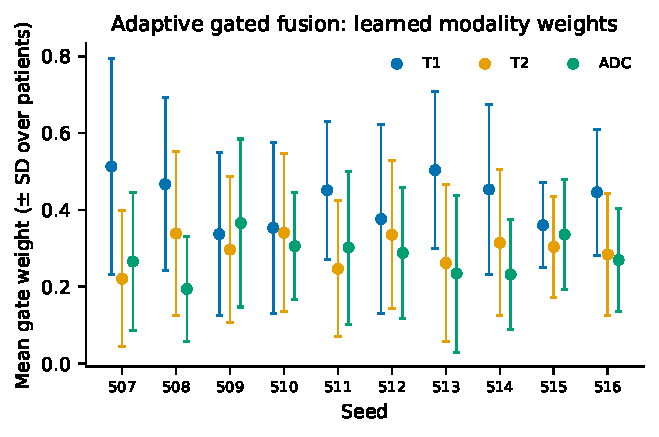
\includegraphics[width=\columnwidth]{figures/fusion_gate_weights.pdf}
\caption{Learned modality weights of the adaptive gated fusion network on harmonized features, per seed (mean $\pm$ SD over training patients).}
\label{fig:gates}
\end{figure}

From an interpretability perspective, the global-weight fusion model tends to assign relatively balanced weights across T1, T2, and ADC modalities (about one third each). On the original features, the gated fusion model learns patient-specific weights whose pattern changes from seed to seed, with T2 receiving between 0.09 and 0.64 of the average weight, consistent with the multiple local optima observed earlier. After harmonization, the gated weights become more consistent across seeds and favor T1 (mean 0.43, compared with 0.29 for T2 and 0.28 for ADC; Fig.~\ref{fig:gates}), in agreement with T1 being the strongest single modality after harmonization.

Across all the supervised models, a consistent pattern emerges: performance appears to saturate, and models consistently underperform in detecting LVI-positive cases, often misclassifying them as negative. The harmonization analysis shows that part of the earlier performance came from acquisition differences that are confounded with the label, and that the LVI signal remaining within a single acquisition batch is modest.

\subsection{Unsupervised Learning}

\begin{figure*}[t]
\centering
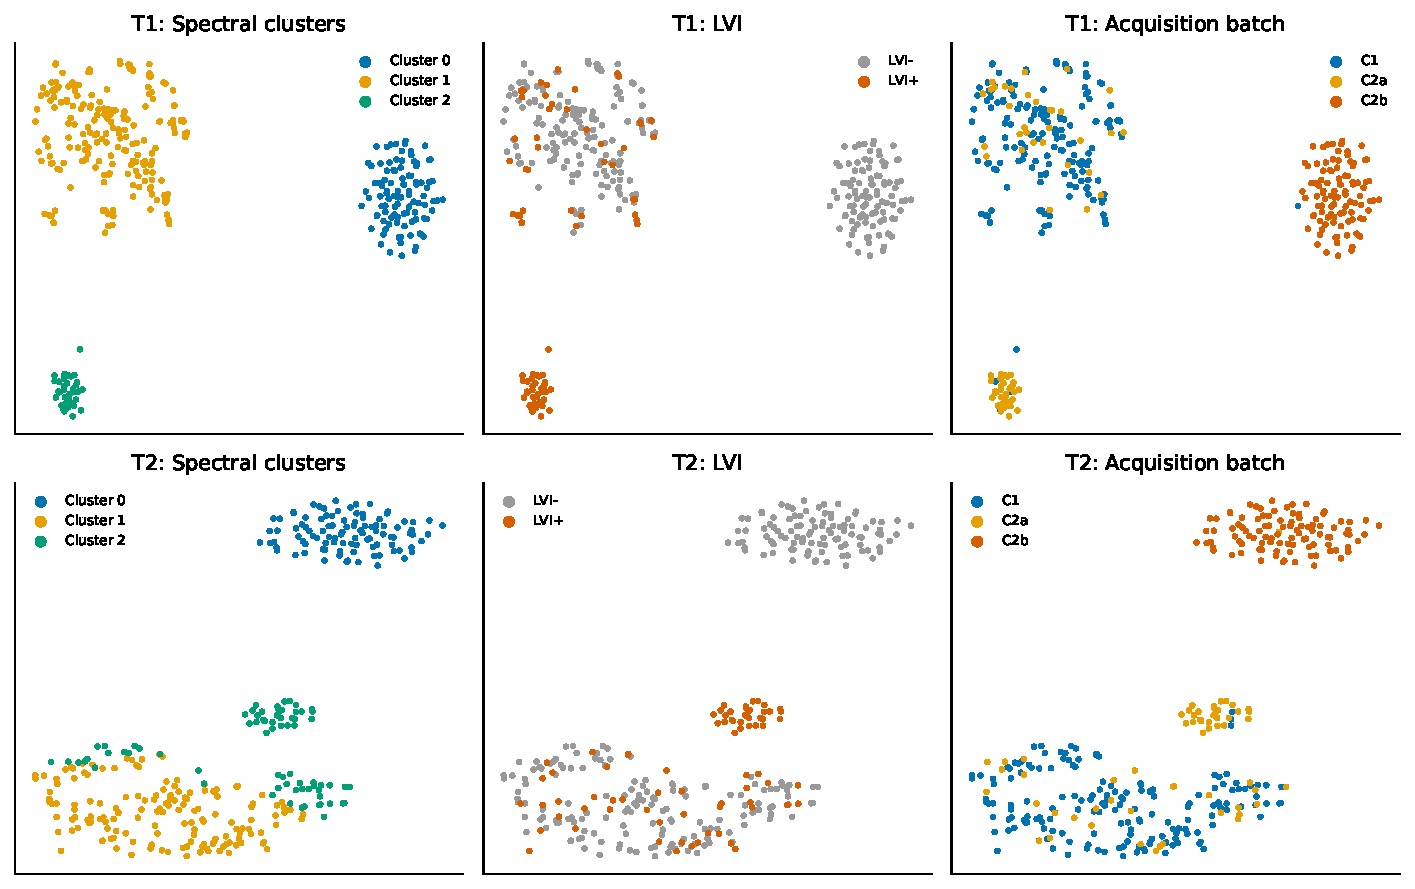
\includegraphics[width=0.85\textwidth]{figures/spectral_tsne_k3_original.pdf}
\caption{Spectral clustering with $K=3$ on the original T1 and T2 features (t-SNE embeddings): cluster assignments (left), LVI status (middle) and acquisition batch (right).}
\label{fig:k3_spectral}
\end{figure*}

\begin{table}[t]
\caption{Spectral clustering stability (mean pairwise ARI / PAC) and Cram\'er's $V$ of the clusters with acquisition batch, $K=3$}
\label{tab:spectral}
\centering
\footnotesize
\begin{tabular}{lcccc}
\toprule
 & \multicolumn{2}{c}{\textbf{Original}} & \multicolumn{2}{c}{\textbf{ComBat (batch)}}\\
\textbf{Modality} & \textbf{ARI / PAC} & \textbf{$V_{\text{batch}}$} & \textbf{ARI / PAC} & \textbf{$V_{\text{batch}}$}\\
\midrule
T1  & 1.00 / 0.00 & 0.81 & 0.48 / 0.51 & 0.09 \\
T2  & 0.93 / 0.05 & 0.76 & 0.57 / 0.43 & 0.32 \\
ADC & 0.94 / 0.06 & 0.76 & 0.52 / 0.49 & 0.37 \\
\bottomrule
\end{tabular}
\end{table}

On the original features, single-modality spectral clustering is highly stable, as previously reported: for $K=2$ all three modalities reach $\text{ARI} = 1$ and $\text{PAC} = 0$, and for $K=3$ T1 remains highly robust ($\text{ARI} \approx 1.00$, $\text{PAC} \approx 0.004$; Table~\ref{tab:spectral}). However, the clusters reproduce the acquisition batches (Fig.~\ref{fig:k3_spectral}). For $K=2$, one cluster is batch C2b (98 of its 99 patients; Cram\'er's $V$ with batch 0.99), which explains why it is purely LVI-negative. For $K=3$, the T1 clusters consist of this C2b cluster, a mixed cluster (196 patients, 22\% LVI-positive, mostly center~1), and a purely LVI-positive cluster of 34 patients, 30 of whom are the center-2 LVI-positive patients that form a separate extraction block.

After harmonization by acquisition batch, this structure disappears. Spectral clustering then mostly separates a few outlying patients from the rest of the cohort, and stability is low for every modality and $K$ (ARI 0.44–0.89, PAC 0.08–0.54). No stable label-pure subgroup remains.

Restricting supervised learning to the mixed T1 cluster of the original features reduces the cross-validated AUC of logistic regression with T1+T2 from 0.88 in the whole cohort to $0.63 \pm 0.09$, close to the center-1-only estimate. This confirms that the mixed region, which contains most center-1 patients, is where the label-related information of the radiomic features is actually weak. A multi-modal latent-space analysis of the harmonized data, with MOFA, $k$-means consensus clustering and post-hoc clinical characterization, is presented in the Unsupervised Extension; it likewise finds only weak cluster structure that is not explained by clinical or pathological variables.

\section{Discussion}

Our results agree with earlier MRI radiomics studies of LVI in endometrial cancer, which reported useful discrimination from T2-weighted, diffusion and contrast-enhanced features with logistic, nomogram or machine-learning models \cite{luo2020multiparametric,long2021mri,liu2024multimodal,ma2025predictive}, but only before harmonization. The central finding of this study is that, in this dataset, a substantial part of the apparent signal is technical. Center~2 contains two acquisition batches, one entirely LVI-negative, and its LVI-positive patients form a separately extracted block. Without accounting for this, models and clusters can separate batches and appear to predict LVI \cite{leek2010tackling}. ComBat by hospital center does not solve the problem, because the technical shift occurs between acquisition runs within a center; this illustrates the recommendation that the batch should be defined by the acquisition setting \cite{orlhac2022guide}.

Harmonization by acquisition batch removes the first- and second-order batch effects and gives more honest estimates, but it cannot fully separate batch from biology. Because batch C2b has no LVI-positive patient, removing its mean shift also removes any true difference between its patients and the rest, and protecting LVI in the ComBat model would instead re-inject the label \cite{nygaard2016methods}. The within-center-1 analysis avoids this problem altogether and suggests that the achievable AUC from these features is around 0.68. The leave-one-center-out results, which range from 0.53 to an implausible 0.98, show that cross-center validation is uninformative when center composition is confounded with the label in this way.

After harmonization, T1 carries the most information, and the previously observed redundancy between T2 and ADC largely disappears. The plateau in performance is informative in itself: linear models matched kernel methods and fusion networks, and the networks overfit the harmonized data. In small-sample multimodal problems, added model capacity mainly increases variance, and late or adaptive fusion helps only when modalities carry complementary signal \cite{pereira2023comparative,baltrusaitis2019multimodal}.

Clinically, the tuned operating point combines high precision with moderate recall. Such a model is better suited to ruling LVI in than to ruling it out. Combining radiomics with readily available clinical and imaging-report variables, such as tumor size, depth of myometrial invasion and the radiologist-measured ADC value, has improved LVI prediction in previous work \cite{ma2025predictive} and is a natural next step.

\section{Conclusion}

In this study, we investigated MRI-based LVI prediction using multi-modal radiomics features through both supervised and unsupervised learning frameworks, with explicit center harmonization. Without harmonization, the T1+T2 combination achieved the best performance (test AUC 0.93), reproducing our earlier results. Harmonization by acquisition batch, fitted on training data only, reduced the cross-validated AUC to about 0.83, and within a single center the AUC was 0.68. Nonlinear models and adaptive gated fusion networks did not improve on simple linear models and overfit the harmonized data.

Through unsupervised clustering analysis, we showed that the stable, label-pure spectral clusters observed on the original features correspond to acquisition batches, and that no stable cluster structure remains after harmonization. The mixed-label region, which contains most center-1 patients, is where the radiomic features carry little LVI information.

Overall, our findings suggest that the performance ceiling in LVI prediction is driven not only by patient-level heterogeneity but also by technical structure in the data. This highlights the importance of identifying acquisition batches, harmonizing within the training data, and validating within batch before interpreting radiomic models in medical imaging tasks.

A key limitation of this study lies in the quality and reliability of the extracted radiomics features. The center-2 batches differ in feature scale by orders of magnitude, suggesting different extraction settings, and cross-file consistency checks reported in the Unsupervised Extension indicate that patient linkage across sequences should be verified against the source records. Errors at this stage cannot be corrected by downstream models.

In addition, the relatively small sample size increases the risk of overfitting and limits the generalizability of the results. Because acquisition batch is confounded with the label, no harmonization method can recover an unbiased estimate from the pooled data; the within-center-1 estimate is unbiased by batch but based on only 169 patients.

Future work will focus on re-extracting features with a common protocol and discretization, harmonizing on recorded scanner and protocol information rather than inferred batches, validating models in an external cohort in which LVI is not linked to acquisition, and incorporating clinical information into combined models.

\section{Reproducibility}
\label{sec:repro}
All code, data and results are available at \texttt{github.com/wpuzhu/STATS507-Coursework}. The script \texttt{run\_all.sh} reproduces every table and figure in this report and in the Unsupervised Extension from the raw feature tables, with fixed random seeds.

\bibliographystyle{IEEEtran}
\bibliography{reference}

\end{document}
